\documentclass{beamer}

\mode<presentation> { \usetheme{gruvbox} }
\setbeamerfont{frametitle}{size=\huge}


\usepackage{graphicx} % Allows including images
\usepackage{booktabs} % Allows the use of \toprule, \midrule and \bottomrule in tables
%\usepackage{listings}             % Include the listings-package
\usepackage{minted}
\usepackage{tikz}
\usepackage{drawstack}
\usetikzlibrary{calc,shapes.callouts,shapes.arrows,chains,positioning,fit,shapes, arrows.meta, arrows}
\usepackage{verbatimbox}
\usepackage{tcolorbox}
\usepackage{forloop}
\usepackage{seqsplit}
\usepackage{bytefield}


\hypersetup{
    colorlinks=true,
}
\usemintedstyle{paraiso-dark}
\graphicspath{ {./images/}{../../slides-source-dep/images/} }
\DeclareGraphicsExtensions{.png,.pdf}

\newcommand{\pointthis}[2]{
    \tikz[remember picture,baseline]{\node[anchor=base,inner sep=0,outer sep=0]%
    (#1) {\underline{#1}};\node[overlay,rectangle callout,%
    callout relative pointer={(0.2cm,0.7cm)},fill=green!50] at ($(#1.north)+(-.5cm,-1.4cm)$) {#2};}%
}%

\newcounter{loopcntr}
\newcommand{\rpt}[2][1]{%
  \forloop{loopcntr}{0}{\value{loopcntr}<#1}{#2}%
}

\newcommand{\hash}[1]{{\ttfamily\seqsplit{#1}}}

\newlength{\bitlabelwidth}
\newcommand{\rotbitheader}[1]{%
  \tiny
  \settowidth{\bitlabelwidth}{\quad 9999}%
  \rotatebox[origin=B]{60}{\makebox[\bitlabelwidth][r]{#1}}%
}

\newenvironment{zerohyphen}
 {\global\chardef\savedhyphenchar=\hyphenchar\font % save the current hyphenchar
  \lefthyphenmin=1 \righthyphenmin=1 % no limits on hyphenation
  \hyphenchar\font=23 }
 {\par\hyphenchar\font=\savedhyphenchar}% eject the paragraph and restore

%----------------------------------------------------------------------------------------
%	TITLE PAGE
%----------------------------------------------------------------------------------------

\title[Introduction to Binary Exploitation]{\huge \textbf{Introduction to Binary Exploitation}} % The short title appears at the bottom of every slide, the full title is only on the title page

\author{Andrew Haberlandt} % Your name
\date{Feburary 23, 2021} % Date, can be changed to a custom date

\begin{document}

{ % this brace groups the background template with just the first slide
\usebackgroundtemplate{%
    \begin{tikzpicture}
        \path [outer color = blue!5, inner color = blue!1]
        (0,0) rectangle (\paperwidth,\paperheight);
        \node[anchor=south west, inner sep=0,line width=0,draw,text width=\paperwidth,fill=almostblack] at (0,0) {\textcolor{darkgray}{\hash{00110110100011010001101101101111100010010111011001110101001111101110100101100101001000001010111000001100110000111010100100001110100010110101001010100001011100000110011111111111100110011010100100101111110111110011101011110010100001001101101010111111011000010110011101110110110000000101101101111110111010111001110010111100110110100100111110111011010110111010101101000011000100011101001011010101111101010000001000001111011111000100111001010000101010000010111001101111101111011111011001110100101101100000011000011110110111010111110001111001110011011110101001001011110001101010110000110110100011000101110110101001110100011101100111101000001001111110000111100010010110000111110101010100000000001110000001010001110110001111000100001100010110101011100011101110101100111111010111101000100111000011110110100011000110111011001101101111111100001010101010010100100101110101011111010110100111011000101010111000010110010010011000010110011000111000110110000010110001100110100011000000111100110110101011100100011110100011011010001101000110110110111110001001011101100111010100111110111010010110010100100000101011100000110011000011101010010000111010001011010100101010000101110000011001111111111110011001101010010010111111011111001110101111001010000100110110101011111101100001011001110111011011000000010110110111111011101011100111001011110011011010010011111011101101011011101010110100001100010001110100101101010111110101000000100000111101111100010011100101000010101000001011100110111110111101111101100111010010110110000001100001111011011101011111000111100111001101111010100100101111000110101011000011011010001100010111011010100111010001110110011110100000100111111000011110001001011000011111010101010000000000111000000101000111011000111100010000110001011010101110001110111010110011111101011110100010011100001111011010001100011011101100110110111111110000101010101001010010010111010101111101011010011101100010101011100001011001001001100001011001100011100011011000001011000110011010001100000011110011011010101110010001111010}}};
    \end{tikzpicture}
}


\begin{frame}
    \titlepage % Print the title page as the first slide
    \begin{tikzpicture}[overlay]
        \node[anchor=south east, yshift=-1cm, xshift=-2cm] (shirt1) at (current page.south east) {
\includegraphics[width=0.15\paperwidth]{logo.png}};
    \end{tikzpicture}
    \begin{itemize}
        \item \textbf{Don't forget to start recording}
        \item Slides are on https://wiki.osucyber.club
        \item \small{Some content adapted from: Nathan Peercy (Purdue)}
    \end{itemize}
\end{frame}
} % end background template


\begin{frame}
    \frametitle{Announcements}
    \begin{itemize}
        \item \textbf{Next Week:} Group solve time focusing on pwn
    \end{itemize}
\end{frame}


\setbeamercolor{background canvas}{bg=almostblack}
\setbeamertemplate{section in toc}[square]
\begin{frame}
    \frametitle{Overview} % Table of contents slide, comment this block out to remove it
    \tableofcontents % Throughout your presentation, if you choose to use \section{} and \subsection{} commands, these will automatically be printed on this slide as an overview of your presentation
\end{frame}


\section{What is binary exploitation?}
\begin{frame}
    \frametitle{What is binary exploitation?}
    \begin{itemize}
        \item{Make a [compiled/binary] program do something it wasn't intended to do}
        \item{Usually this means the goal is arbitrary code execution}
        \item{pwn is awesome but pwn is hard. You'll eventually need a good understanding of:}
        \begin{itemize}
            \item{Assembly (we'll use x86)}
            \item{C}
            \item{Operating systems}
        \end{itemize}
    \end{itemize}
\end{frame}


\begin{frame}
    \frametitle{Why}
    \begin{itemize}
        \item{Native code is everywhere}
        \item{No really, EVERY APPLICATION EVER ULTIMATELY ENDS UP RUNNING MACHINE CODE}
    \end{itemize}
\end{frame}


\begin{frame}
    \begin{tikzpicture}[overlay]
        \node[anchor=south east, yshift=-5cm, xshift=-4cm] (turtle) at (current page.south east) {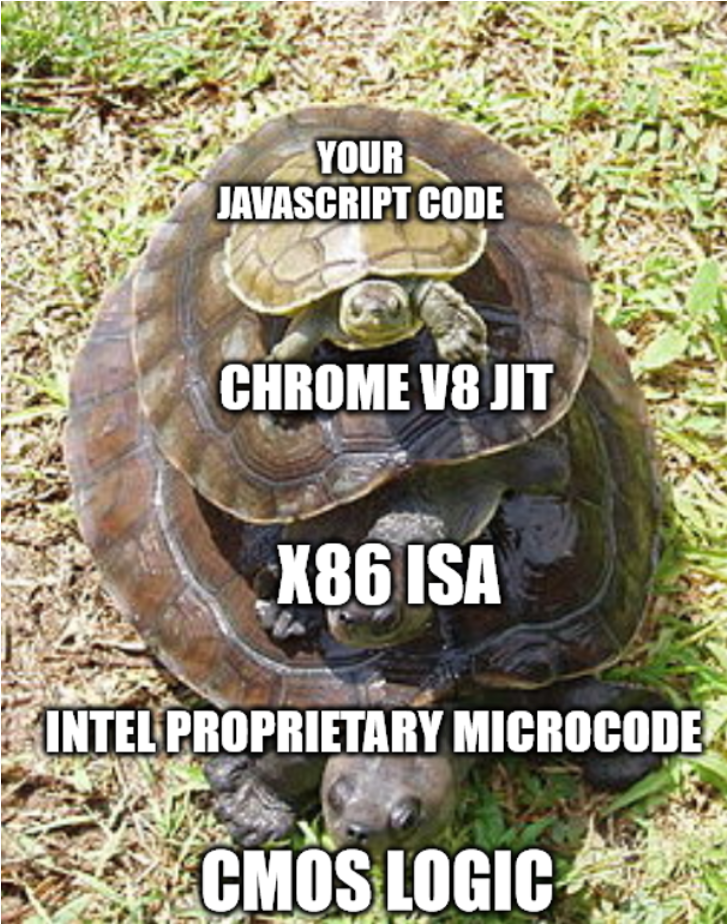
\includegraphics[width=0.5\paperwidth]{turtle.png}};
        \node[below=of turtle] {\tiny{Meme credit: Stephen Tong of Georgia Tech's Greyhat Club}};
    \end{tikzpicture}
\end{frame}


\begin{frame}
    \frametitle{Why}
    \begin{itemize}
        \item{GOAL: Take over ('pwn') a machine}
        \begin{itemize}
            \item{We want \textbf{Arbitrary Code Execution}. If you can run whatever code you want, you can do anything the OS allows that process to do (usually anything the user can do)}
            \item{After you have code execution, \textbf{privilege escalation} concerns exploiting (usually) the operating system to gain additional privileges (i.e. normal user root access, or sometimes directly to kernel code execution)}
            \item{Some special programs (ie. sudo) are usually given extra privileges to run as root ("suid programs"); exploit one of these and your code runs as root}
            \item{Examples: bug bounties like \href{https://hackerone.com/valve?type=team}{Valve}, \href{https://bugcrowd.com/tesla}{Tesla}, many others}
        \end{itemize}
    \end{itemize}
\end{frame}


\begin{frame}
    \frametitle{What does it look like to 'pwn' a machine?}
    \begin{itemize}
        \item{\textbf{Real-life examples}}
        \begin{itemize}
            \item{Buffer overflow in CSGO/Half-Life/TF2 client, allowing a malicious server to run code just by viewing the server's info https://hackerone.com/reports/470520}
            \item{Read an arbitrary file on a Half-Life server: https://hackerone.com/reports/590279}
        \end{itemize}
        \item{\textbf{Arbitrary code execution}}
        \begin{itemize}
            \item{Often demonstrated by: getting a shell}
            \item{``popping calc"}
            \item{Sometimes in CTF problems: opening and reading a special 'flag' file is sufficient (can do with shell, or not)}
            \item{After you have code execution, you're often done unless you're the NSA or CIA}
        \end{itemize}
    \end{itemize}
\end{frame}


\begin{frame}
    \frametitle{Demo 1: Reverse shell in Bash}
\end{frame}


\section{How to get code execution}
\subsection{Common vulnerabilities}
\begin{frame}
    \frametitle{Common vulnerabilities}
    \begin{itemize}
        \item{Command injection}
        \item{Memory corruption: a broad category}
        \item{Off-by-one errors}
        \item{Race conditions}
        \item{(lack of) Input validation}
        \item{Miscellaneous logic bugs}
    \end{itemize}
\end{frame}


\subsection{Command Injection}
\begin{frame}[fragile]
    \frametitle{Command Injection}
    \begin{itemize}
        \item{Programmers are lazy and often 'shell out' to run another program}
        \item{If an attacker controls part of the command being run, they can use features of the shell (usually bash) to end the previous command and inject their own}
    \end{itemize}
    \begin{minted}[tabsize=2, fontsize=\footnotesize]{c}
#include <stdio.h>
void get_log_file(char *name) {
  char cmd[50];
  sprintf(cmd, "cat log_file_%s", name);
  system(cmd);
}
    \end{minted}
    \begin{itemize}
        \item{ie. if you can cause the program to call get\_log\_file with something like\linebreak\texttt{; cat /etc/passwd}\linebreak then you can run other commands}
    \end{itemize}
\end{frame}

\begin{frame}
    \frametitle{Demo 2: Command injection}
\end{frame}


\subsection{Logic Bugs}
\begin{frame}
    \frametitle{Logic Bugs}
    \begin{itemize}
        \item{Most are unintentional, Intentional logic bugs are essentially "backdoors".}
        \item{Leaving in debug options: ex. bypass access control by adding debug=1}
        \item{Program gets confused about state when receiving packets/commands out-of-order}
        \item{An example: "[steam client] Opening a specific steam:// url overwrites files at an arbitrary location" https://hackerone.com/reports/667242}
    \end{itemize}
\end{frame}


\subsection{Memory Corruption Bugs}
\begin{frame}[fragile]
    \frametitle{Memory Corruption Bugs}
    \begin{itemize}
        \item{Memory is a byte-addressable array of bytes}
        \item{If a user can write somewhere they are not intended to, it can be the cause of a memory corruption bug}
        \item{Everything has a finite size}
    \end{itemize}
    \vspace{5mm}
    \begin{bytefield}[bitwidth = 1.5em, leftcurly = .]{16}
        \bitheader[bitformatting=\rotbitheader, lsb=1000, endianness = little]{1000-1015}\\
        \bytefieldsetup{}%
        \begin{leftwordgroup}{Memory}
		      \bitboxes*{1}{{47} {6F} {20} {42} {75} {63} {6B} {72} {00} {00} {00} {00} {E8} {03} {00} {00} }
        \end{leftwordgroup}\\[1ex]
        \begin{leftwordgroup}{}
		      \bitbox{9}{"Go Bucks", null-terminated} & \bitbox{3}{} & \bitbox{4}{\small{Addr (0x3E8)}\\ \tiny{(Little endian)}}
        \end{leftwordgroup}\\[1ex]
    \end{bytefield}
\end{frame}

\begin{frame}[fragile]
    \frametitle{Memory Corruption Bugs}
    \begin{itemize}
        \item{String Functions and length-checks}
        \begin{itemize}
            \item{\textbf{strcpy / strncpy:} Arguments are two pointers, copies all characters from one location to the other until it reaches a null byte}
            \item{\textbf{gets / fgets:} Reads a string from the user (gets uses stdin, fgets can use any file)}
            \item{\textbf{others: } Most other string functions rely on the strings being terminated by a null byte and many don't check length}
        \end{itemize}
    \end{itemize}
\end{frame}

\begin{frame}[fragile]
    \frametitle{Memory Corruption Bugs}
    \begin{columns}
    \begin{column}{0.5\textwidth}
        \begin{itemize}
            \item{The important question is ``can we overwrite anything important?"}
            \begin{itemize}
                \item{To answer, need to know some things about where stuff is in memory}
            \end{itemize}
            \item{Every function starts by making room for it's own local variables on the stack}
        \end{itemize}
    \end{column}
    \begin{column}{0.5\textwidth}
        \begin{drawstack}[scale=.5, text=invtext]
            \tiny % can also use any from https://tex.stackexchange.com/questions/107057/adjusting-font-size-with-tikz-picture
            \stacktop{}
            \startframe
            \padding{0}{} \cellcom{base - 44}
            \padding{4}{char input[32]} 
            \cell{int \textit{c}} \cellcom{base - 12}
            \cell{int \textit{b}} \cellcom{base - 8}
            \cell{int \textit{a}} \cellcom{base - 4}
            \cell{base pointer for main()} \cellptr{base}
            \bcell{Return addr into main()} \cellcom{base + 8}
            \finishframe{function \\ {\tt foo ()}}
            \startframe
            \cell{Saved base pointer} \cellptr{base}
            \bcell{Return address} \cellcom{base + 8}
            \finishframe{function \\ {\tt main ()}}
            \stackbottom{}
        \end{drawstack}
    \end{column}
    \end{columns}
\end{frame}


\begin{frame}[fragile]
    \frametitle{Simplest example: Stack buffer overflow into another variable}
    \begin{minted}[tabsize=2, fontsize=\footnotesize]{c}
int main() {
  char buf1[16];
  char buf2[16];

  // get a (arbitrary-length) string from the user
  gets(buf1);

  // print the strings back to the user
  printf("buf1: %s\n", buf1);
  printf("buf2: %s\n", buf2);

  // check for win condition
  if (strcmp(buf2, "win") == 0) {
    system("/bin/sh");
  }
}
    \end{minted}
\end{frame}

\begin{frame}[fragile]
    \frametitle{Simplest example: Stack buffer overflow into another variable}
    \begin{columns}
    \begin{column}{0.5\textwidth}
        \begin{itemize}
            \item{We can change the value of other variables on the stack!}
        \end{itemize}
    \end{column}
    \begin{column}{0.5\textwidth}
        \begin{drawstack}[scale=.5, text=invtext]
            \tiny % can also use any from https://tex.stackexchange.com/questions/107057/adjusting-font-size-with-tikz-picture
            \stacktop{} \cellcomL{Low Addresses}
            \startframe
            \padding{4}{char buf1[16]} 
            \padding{4}{char buf2[16]} 
            \finishframe{function \\ {\tt main ()}}
            \padding{0}{} \cellcomL{High Addresses}
        \end{drawstack}
    \end{column}
    \end{columns}
\end{frame}

\begin{frame}
    \frametitle{Demo: Stack buffer overflow and pwntools}
\end{frame}

\begin{frame}[fragile]
    \frametitle{OK, but we want code execution}
    \framesubtitle{Stack buffer overflow into return address}
    \begin{columns}
    \begin{column}{0.5\textwidth}
    \begin{minted}[tabsize=2, fontsize=\footnotesize]{c}
int main() {
    char buf1[16];

    // get a (arbitrary-length)
    // string from user
    gets(buf1);
}
    \end{minted}
    \end{column}
    \begin{column}{0.5\textwidth}
        \begin{drawstack}[scale=.5, text=invtext]
            \tiny % can also use any from https://tex.stackexchange.com/questions/107057/adjusting-font-size-with-tikz-picture
            \stacktop{} \cellcomL{Low Addresses}
            \startframe
            \padding{0}{}
            \padding{4}{char buf1[16]}
            \cell{Saved RBP} \cellcomL{Address of caller's stack frame base}
            \bcell{Return addr} \cellcomL{Address to jump to, in caller}
            \finishframe{function \\ {\tt main ()}}
            \draw[->, line width=0.5mm, xshift=-3cm, yshift=-1cm, color=red] (0,0) -- (0,-2) node[midway, left, text=red] {Writes toward high addresses};
        \end{drawstack}
    \end{column}
    \end{columns}
\end{frame}


\begin{frame}
    \frametitle{1990s exploitation}
    \begin{itemize}
        \item{You control where the program goes when the current function returns}
        \item{Just put your code somewhere you know the address of, and then overwrite the return address so that it holds the address of your code}
        \item{When the function returns, your code runs}
    \end{itemize}
\end{frame}


\begin{frame}
    \frametitle{Demo 3: Return to the 1990s + pwntools}
\end{frame}


\subsection{ROP}
\begin{frame}
    \frametitle{Modern memory protections have entered the chat}
    \begin{itemize}
        \item{You can't just write your code onto the stack and jump to it. The stack is not normally executable.}
        \item{We need to be more creative}
    \end{itemize}
\end{frame}


\begin{frame}[fragile]
    \frametitle{ROP}
        \begin{columns}
            \begin{column}{0.5\textwidth}
                \begin{itemize}
                    \item{We don't just control the return address, we can keep writing and we control the whole stack}
                    \item{We can return to specific locations that do useful things and then return again ('gadgets')}
                    \begin{itemize}
                        \item{pop rdi; ret;}
                        \item{pop rdx; pop rax; ret;}
                    \end{itemize}
                    \item{Chain these together to control all registers and you can eventually make syscalls, etc.}
                \end{itemize}
            \end{column}
            \begin{column}{0.5\textwidth}
                \begin{drawstack}[scale=.5, text=invtext]
                    \tiny % can also use any from https://tex.stackexchange.com/questions/107057/adjusting-font-size-with-tikz-picture
                    \stacktop{} \cellcomL{Low Addresses}
                    \startframe
                    \padding{0}{}
                    \padding{4}{char buf1[16]}
                    \cell{Saved RBP} \cellcomL{Address of caller's stack frame base}
                    \bcell{Return addr} \cellcomL{Address to jump to}
                    \finishframe{function \\ {\tt main ()}}
                    \bcell{evil data} \cellcomL{Whatever your gadget needs on the stack}
                    \bcell{Return addr} \cellcomL{ANOTHER address to jump to}
                    \bcell{evil data} \cellcomL{Whatever your gadget needs on the stack}
                    \bcell{evil data} \cellcomL{Whatever your gadget needs on the stack}
                    \bcell{Return addr} \cellcomL{ANOTHER address to jump to}
                \end{drawstack}
            \end{column}
            \end{columns}
\end{frame}


\begin{frame}
    \frametitle{More on ROP}
    \begin{itemize}
        \item{https://docs.pwntools.com/en/dev/rop/rop.html}
        \item{If there is interest we may do another ROP talk}
    \end{itemize}
\end{frame}

\begin{frame}
    \frametitle{More examples of memory corruption}
    \begin{itemize}
        \item{Some memory bugs can lead to arbitrary read/write}
        \begin{itemize}
            \item{Can you overwrite an entry in the Global Offset Table (GOT) - addresses of code in dynamically-loaded libraries}
            \item {Can you leak the address of something else important?}
        \end{itemize}
        \item{Controlled array index}
        \begin{itemize}
            \item{You can read/write beyond the bounds of an array, without corrupting everything in between.}
        \end{itemize}
    \end{itemize}
\end{frame}


\begin{frame}
    \frametitle{Common Defenses}
    \begin{itemize}
        \item{ASLR - Address Space Layout Randomization}
        \item{PIE - Position Independent Executable (DEMO?)}
        \item{NX - Non-eXecutable memory}
        \item{Stack Canaries}
        \item{Many more...}
    \end{itemize}
\end{frame}


\section{Useful Tools, Recommended Challenges, Next Week}
\begin{frame}
    \frametitle{Useful Tools}
    \begin{itemize}
            \item{GDB with GEF, pwndbg}
            \item{Ghidra and RE tools}
            \item{python3 with pwntools}
            \item{checksec, ROPGadget, Ropper}
    \end{itemize}
\end{frame}


\begin{frame}
    \frametitle{Recommended Challenges}
    \begin{itemize}
        \item{\textbf{speedrun series}: 8-100 points, starts from basics and gradually becomes more difficult/more modern}
        \item{\textbf{speedrun0, 0.25, 0.5, and 1} are \textit{very} similar to what was demoed today, it progresses from there in small steps}
    \end{itemize}
\end{frame}


\begin{frame}
    \frametitle{Next Week}
    \begin{itemize}
        \item{\textbf{Highly Recommended: } Attempt some pwn challenges and have questions ready to go}
        \item{\url{https://bootcamp.osucyber.club/}}
    \end{itemize}
\end{frame}


\end{document}
